\documentclass{beamer}

\mode<presentation>
{
%\usetheme{Warsaw} %ok
%\usetheme{Rochester}
%\usetheme{Madrid}
%\usetheme{Pittsburgh}
%\usetheme{Antibes}
%\usetheme{Montpellier}
%\usetheme{Berkeley}
%\usetheme{PaloAlto}
%\usetheme{Goettingen}
%\usetheme{Marburg}
%\usetheme{Hannover}
%\usetheme{Berlin}
%\usetheme{Ilmenau}
%\usetheme{Dresden}
%\usetheme{Darmstadt}
\usetheme{Frankfurt} %ok
%\usetheme{Singapore} %ok
%\usetheme{Szeged}
%\usetheme{Copenhagen} %ok
%\usetheme{Malmoe}
\setbeamercovered{transparent}
}
% Choose color scheme
%
%\usecolortheme{default}
%\usecolortheme{sidebartab}
%\usecolortheme{albatross}
%\usecolortheme{beetle} 
%\usecolortheme{crane}
%\usecolortheme{dove} 
%\usecolortheme{fly} 
%\usecolortheme{seagull}
%\usecolortheme{lily}
\usecolortheme{orchid}
%
\usepackage{graphicx}
\usepackage[english]{babel}
\usepackage[utf8]{inputenc}

%==============================================================================

\title{Recognizing human actions in still images:
a study of bag-of-features and part-based
representations}
\author{Vincent Delaitre, Ivan Laptev and Josef Sivic}

\begin{document}

\maketitle

%==============================================================================
\begin{frame}
\tableofcontents
\end{frame}

%==============================================================================
\section{Introducing a new dataset}
\begin{frame}
\frametitle{Introducing a new dataset}
We collected a new challenging dataset for real-life human actions. 

It is composed of 968 images collected from Flickr representing natural variations in terms of 
camera view-point, human pose, clothing, occlusions and scene background.

Pictures are distributed among 7 different classes: 
\begin{itemize}
\item Interacting with a computer
\item Taking a photograph
\item Playing music
\item Riding bike
\item Riding horse
\item Running
\item Walking
\end{itemize}

\end{frame}

%------------------------------------------------------------------------------

\begin{frame}
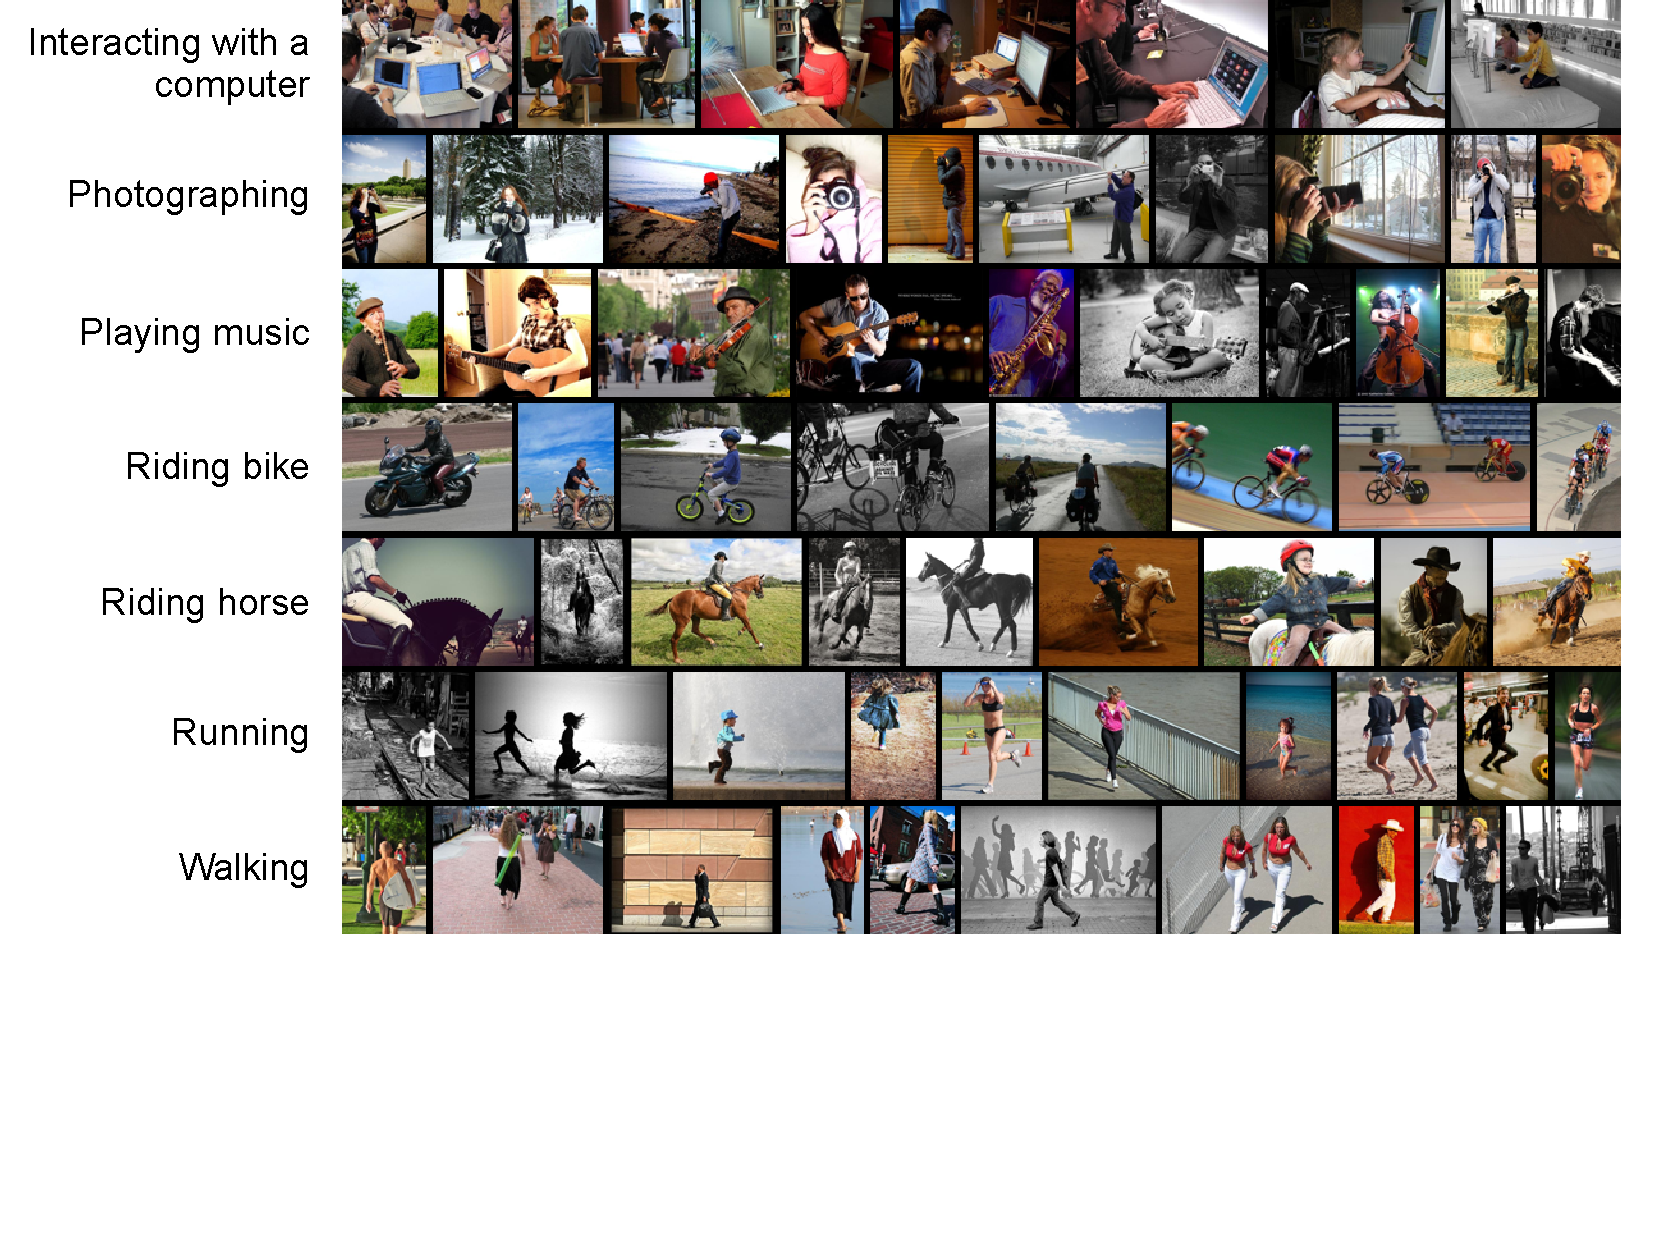
\includegraphics[width=1\linewidth]{figs/my_dataset_cropped.pdf}
\end{frame}

%------------------------------------------------------------------------------

\begin{frame}
\frametitle{Classification task}
Each person is annoted with a bounding box (smallest rectangle containing its visible pixels)
and the action being executed.

\vspace{0.3cm}
In the following, we are interessted in the 7-class classification problem.
The training set consists in 70 images of each type of action, so that at least 48 images
per class remain for test.

\vspace{0.3cm}
We mesure the performances using:
\begin{enumerate}[i]
\item {\em the classification accuracy}: average of the diagonal of the confusion table
\item {\em the mean average precision (mAP)}: mean area under the precision-recall curve of each 1-vs-all classifiers.
\end{enumerate}

\end{frame}

%------------------------------------------------------------------------------

%==============================================================================
\section{Bag-of-features classifier}
\subsection{Image representation}
\subsection{Investigated Kernels}
\subsection{Dealing with bounding boxes}
\begin{frame}

\end{frame}


%==============================================================================
\section{Discriminatively trained part-based model}
\begin{frame}

\end{frame}


%==============================================================================
\section{Experimental results}
\begin{frame}

\end{frame}


\end{document}
